% Gemini theme
% https://github.com/anishathalye/gemini

\documentclass[final]{beamer}

% ====================
% Packages
% ====================

\usepackage[T1]{fontenc}
\usepackage{lmodern}
%\usepackage[size=custom,width=120,height=72,scale=1.0]{beamerposter}
\usepackage[size=a0,orientation=portrait]{beamerposter}
\usetheme{gemini}
\usecolortheme{gemini}
\usepackage{graphicx}
\usepackage{booktabs}
\usepackage{tikz}
\usepackage{pgfplots}
\usepackage{physics}
\usepackage{natbib}
\usepackage{siunitx}

\graphicspath{{Figures/}} %Position of figures, pictures, etc

% ====================
% Lengths
% ====================

% If you have N columns, choose \sepwidth and \colwidth such that
% (N+1)*\sepwidth + N*\colwidth = \paperwidth
\newlength{\sepwidth}
\newlength{\colwidth}
%\setlength{\sepwidth}{0.025\paperwidth}
%\setlength{\colwidth}{0.3\paperwidth}
\setlength{\sepwidth}{0.04\paperwidth}
\setlength{\colwidth}{0.44\paperwidth}

\newcommand{\separatorcolumn}{\begin{column}{\sepwidth}\end{column}}

% ====================
% Title
% ====================

\title{Sensitivity of Oceanic Fronts to nonlinearities of equation of
state investigated using Numerical Experiments}

\author{Romain Caneill \inst{1} \and Fabien Roquet \inst{1}
  \and Gurvan Madec \inst{2} \and Jonas Nycander \inst{3}}

\institute[shortinst]{\inst{1} University of Gothenburg, Sweden
  \samelineand \inst{2} LOCEAN-IPSL Sorbonne university, France
  \samelineand \inst{3} Stockholm University, Sweden}

% ====================
% Footer (optional)
% ====================

\footercontent{
  \href{https://github.com/rcaneill/DRAKKAR-2020-poster}
       {https://github.com/rcaneill/DRAKKAR-2020-poster} \hfill
%%  DRAKKAR, Grenoble, 2020 \hfill
  \href{mailto:romain.caneill@gu.se}{romain.caneill@gu.se}}
% (can be left out to remove footer)

% ====================
% Logo (optional)
% ====================

% use this to include logos on the left and/or right side of the header:
 \logoright{
\includegraphics[height=7cm]{gulogo_inverted}}
% \logoleft{\includegraphics[height=7cm]{logo2.pdf}}

% ====================
% Body
% ====================

\begin{document}

\begin{frame}[t]
\begin{columns}[t]
\separatorcolumn

\begin{column}{1.3\colwidth}
  \vspace{1.65cm}
  \begin{block}{Context}
    Transition zones between saline warm subtropical water and
    cold fresh subpolar water arise
    abruptly. These boundaries are called oceanic fronts
    and have similar structures in the North
    Atlantic Ocean, the North Pacific Ocean and
    the Southern Ocean, suggesting that the same
    processes lead to these frontal structures.
    The nonlinearities of
    the equation of state for seawater -- the
    relation that gives density as a function of
    pressure, salinity, and temperature --
    are expected to constraint these fronts.
    To test this hypothesis, we are developing
    an idealized triple-gyre configuration with the
    ocean global circulation model NEMO (Nucleus for
    European Modelling of the Ocean). This
    configuration includes a continental slope
    along the coastline with a terrain following
    coordinate, except at the equator where an open
    boundary with a no meridional flow
    condition is imposed.
  \end{block}

  \begin{alertblock}{Objectives}
    \begin{itemize}
    \item We analyzed the sensitivity of transition zones to perturbations of the
      nonlinear equation of state.
    \item We ran 5 experiments, varying the cabbeling
      parameter $\lambda_1$ from $3.952 \cdot 10^{-2}$ to $7.952 \cdot 10^{-2}$
      \,$(^\circ\text{C})^{-1}$, and analyzing the resulting
      stratification and circulation.
    \item We are building a reference NEMO triple gyre configuration.
    \end{itemize}
  \end{alertblock}

  \begin{block}{The basin configuration}
    \fbox{
      \begin{minipage}{.33\textwidth}
        \heading{Description of the grid}
        \begin{itemize}
        \item Mercator grid
        \item Continental slopes (2\,km deep at the coast, 4\,km
          deep at the bottom)
        \item Coarse resolution (for the moment)
        \item 36 vertical levels
        \item Terrain following vertical coordinates
        \item Symmetry condition at the equator (no meridional flux)
        \end{itemize}
        
        \begin{figure}
        \centering
        \includegraphics[width=\textwidth]{raw_bathy}
        \caption{Bathymetry of the basin.}
      \end{figure}
    \end{minipage}}
    \hfill
    \fbox{
      \begin{minipage}{.62\textwidth}
        \heading{Description of the forcing fields}
        \begin{minipage}{.6\textwidth}
          \begin{itemize}
          \item Restoring temperature
          \item Penetrative solar radiation
          \item Restoring salinity (used here) or E-P flux
          \item Zonal wind stress
          \end{itemize}
        \end{minipage}
        %% \begin{minipage}{.45\textwidth}
        %%   \begin{center}
        %%     \small
        %%     Definition of the analytical fields.
            
        %%     
\includegraphics[width=2in]{qr-forcing}
        %%   \end{center}
        %% \end{minipage}
        
        
        %% \begin{align}
        %%   T^*(\varphi) &= 25 \cdot \cos\qty(\frac{\pi  \varphi}{2  \phi_N})^2 \\
        %%   S^*(\varphi) &= 37.12 \cdot \exp\qty(-\qty(\frac{\varphi}{260})^2)
        %%   - 1.1 \cdot \exp\qty(-\qty(\frac{\varphi}{7.5})^2) \\
        %%   \tau_x(\varphi) &= 0.1 \cdot \qty[- \cos(\frac{3 \pi \varphi}{2 \phi_N})
        %%   + 0.8 \cdot \exp(-(\frac{\varphi}{5.77})^2) ]
        %% \end{align}

        \heading{Resulting fields}
        \begin{figure}
        \centering
        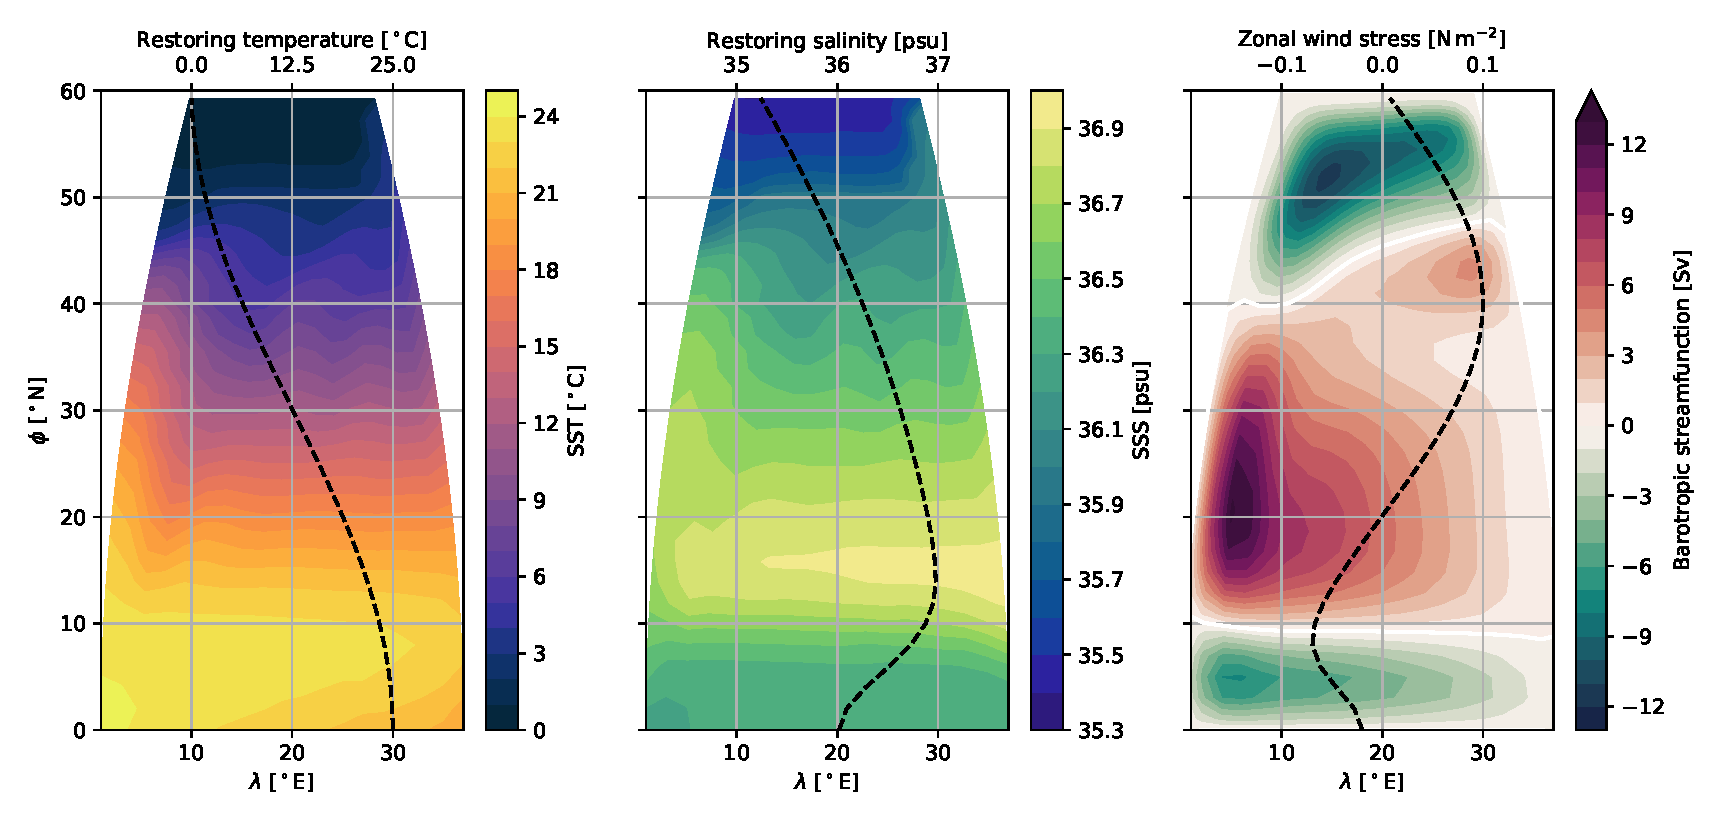
\includegraphics[width=\textwidth]{surf}
        \caption{Sea Surface Temperature, Sea Surface Salinity, Barotropic
          Streamfunction. The forcing fields are represented in dashed lines.}
      \end{figure}
    \end{minipage}}
  
  \end{block}


  
  \begin{alertblock}{Results}
    \begin{minipage}{.35\textwidth}
      \begin{figure}
        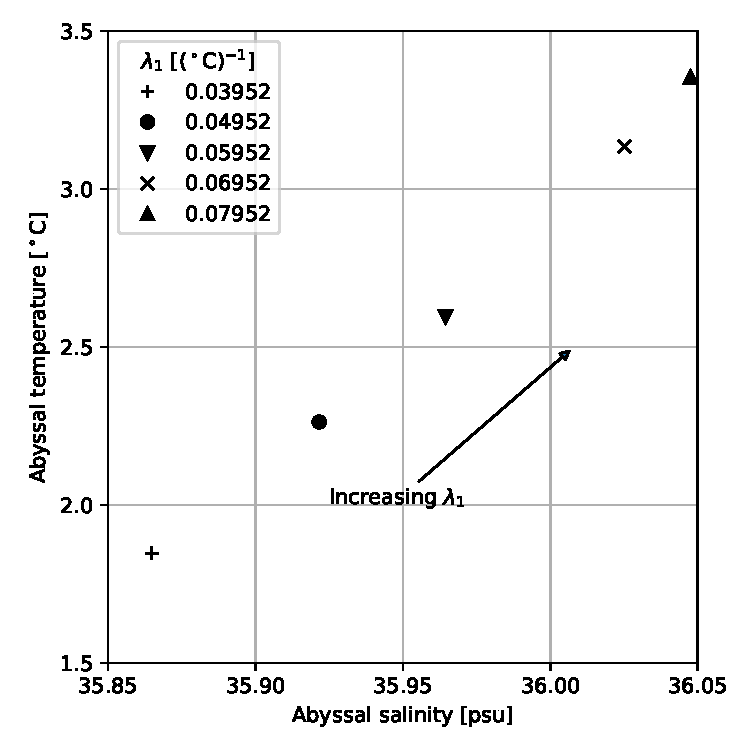
\includegraphics[width=5in]{abyssal}
        \caption{$T$-$S$ diagram for the abyssal water for the fives values of $\lambda_1$.
          Both the temperature and the salinity increase with $\lambda_1$:
          the convective region is displaced to the south.}
      \end{figure}

      \begin{figure}
        \centering
        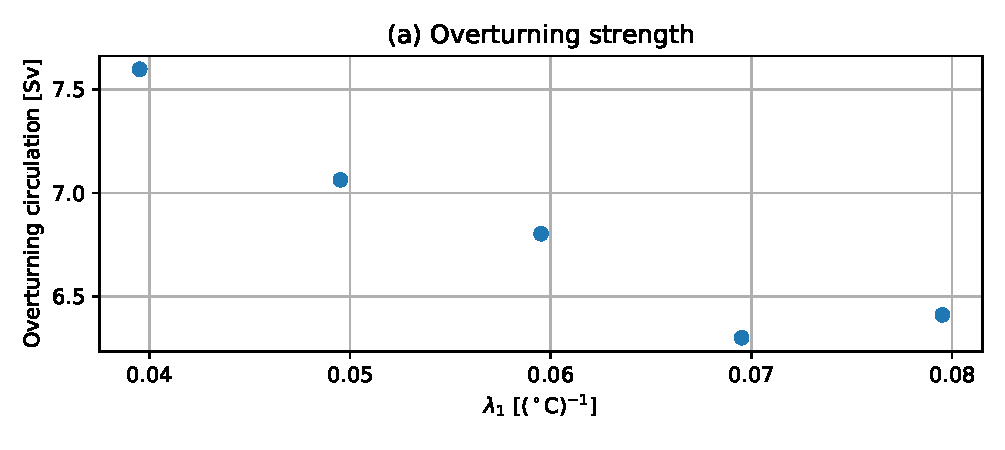
\includegraphics[width=6.7in]{oc_vs_eos}
        \\
        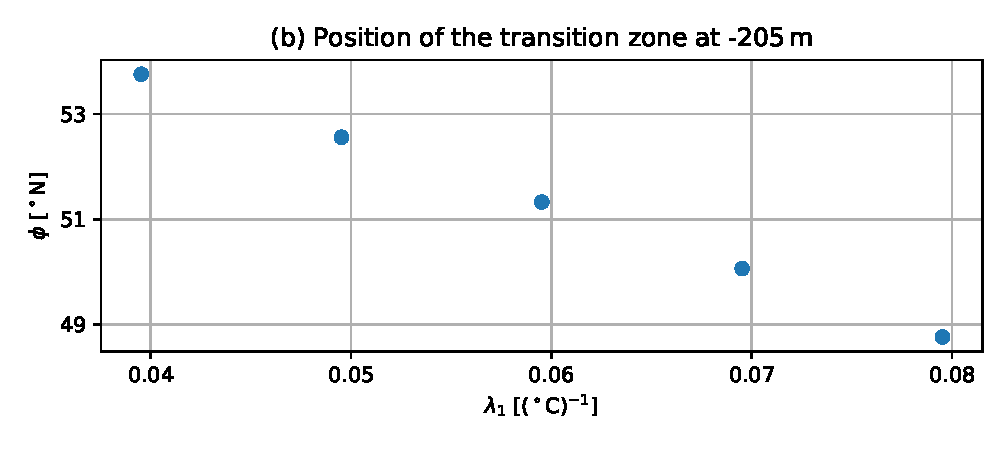
\includegraphics[width=6.7in]{beta_pos}
        \caption{(a) Overturning strength function of the cabbeling term $\lambda_1$.
          The overturning circulation decreases when cabbeling is more important.
          (b) Position of the transition zone at a depth of 205\,m and a longitude of
          23\,$^\circ$E.
          The transition zone corresponds to the northern part of the convective region,
          and its latitude decreases when $\lambda_1$ increases, leading to the
          change of abyssal water properties.}
      \end{figure}
    \end{minipage}
    \begin{minipage}{.6\textwidth}
      \begin{figure}
        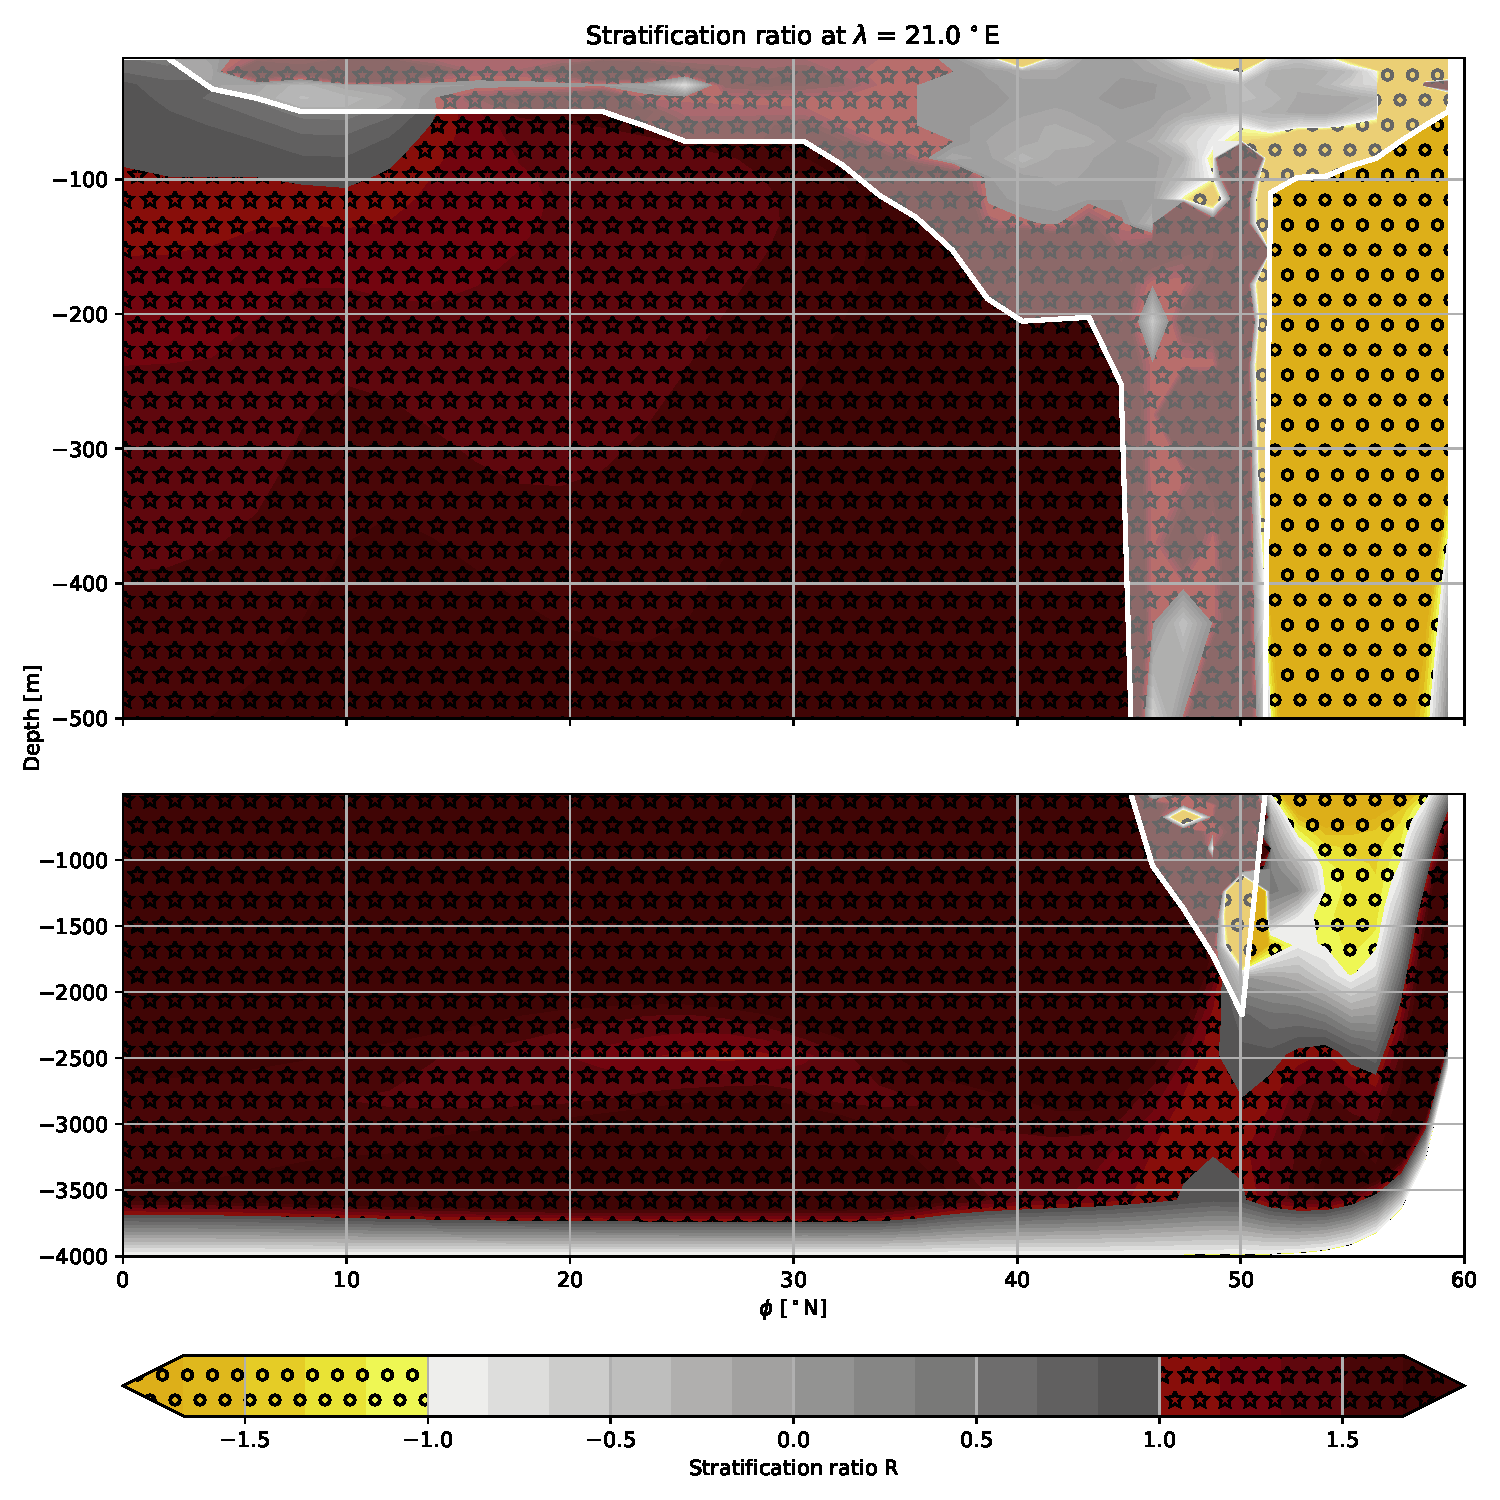
\includegraphics[width=\textwidth]{R_section}
        \caption{Section of the stratification ratio. The red colors (star background)
          represent alpha-ocean
          stratified by the temperature only,
          the yellow areas (round background) are the beta-ocean stratified
          by the salinity only and
          the gray zones are doubly stratified.
          The white line represents the diagnostic mixed layer depth
          and the white dashed area is the mixed layer.}
      \end{figure}

      \heading{Conclusion}%{Take home message}
        With the increase of the cabbeling parameter $\lambda_1$, the stratification
        becomes less sensitive to the temperature more south in the basin.
        As the northern area is stabilized by a strong halocline due to
        fresh surface water, the salinity control of the stratification
        pushes the transition zone to the south. This is accompanied
        by a more southern convection zone and thus a creation of warmer
        and saltier deep water.
        An unexpected effect is the reduction of the overturning strength
        with cabbeling.
    \end{minipage}
    
  \end{alertblock}

\end{column}

\separatorcolumn

\begin{column}{0.7\colwidth}
  \vspace{1.65cm}
  \begin{exampleblock}{Thermodynamic properties}
    \heading{The nonlinear equation of state}
    We use the simplified nonlinear equation of state proposed
    by \citet{roquet_defining_2015}.

    \begin{align}
      \rho(\Theta, S_A, Z) &= \overline{\rho}(Z)
      - \frac{C_b}{2} \qty(\Theta - \Theta_0)^2
      - T_h Z \Theta
      + b_o S_A
    \end{align}

    The term $\overline{\rho}(Z)$ does not play a role in the
    ocean dynamics.

    %% \begin{align}
    %%   \overline{\rho}(Z) &= \rho_0 - b_0 S_0 + \frac{a_0^2}{2 C_b}
    %%   + T_h Z T_0
    %% \end{align}

    \begin{align}
      \alpha = \frac{1}{\rho_0} \qty[C_b (\Theta - \Theta_0) + T_h Z]
      \qand
      \beta = \frac{b_0}{\rho_0}
    \end{align}
    
    \heading{The stratification ratio}
    The stratification ratio $R$ determines if the water column is stratified
    by the temperature only ($R>1$), by the salinity only ($R<-1$) or doubly
    stabilized ($-1 \leq R \leq 1$).
    \begin{align}
      R &= \frac{N_\Theta^2 - N_{S_A}^2}{N^2}
      = \frac{\alpha \pdv{\Theta}{z} + \beta \pdv{S_A}{z}}
      {\alpha \pdv{\Theta}{z} - \beta \pdv{S_A}{z}}
    \end{align}
    
    The thermal expansion $\alpha$ is proportional to the temperature
    (cabbeling effect) while the haline contraction is constant.    
    Thus on warm and tempered regions, the stratification is mainly controlled
    by the temperature (alpha-ocean \citep{carmack_alpha/beta_2007}).
    But at high latitude, the lower value of $\alpha$ associated
    with the halocline lead to a salinity controlled stratification (beta-ocean).

    A $T$-$S$ profile with a stratification ratio $R<-1$ can become unstable when
    the cabbeling term is perturbed, leading to a different polar stratification:
    the nonlinearities of the equation of state are an essential parameter.
    
   
    \begin{figure}
      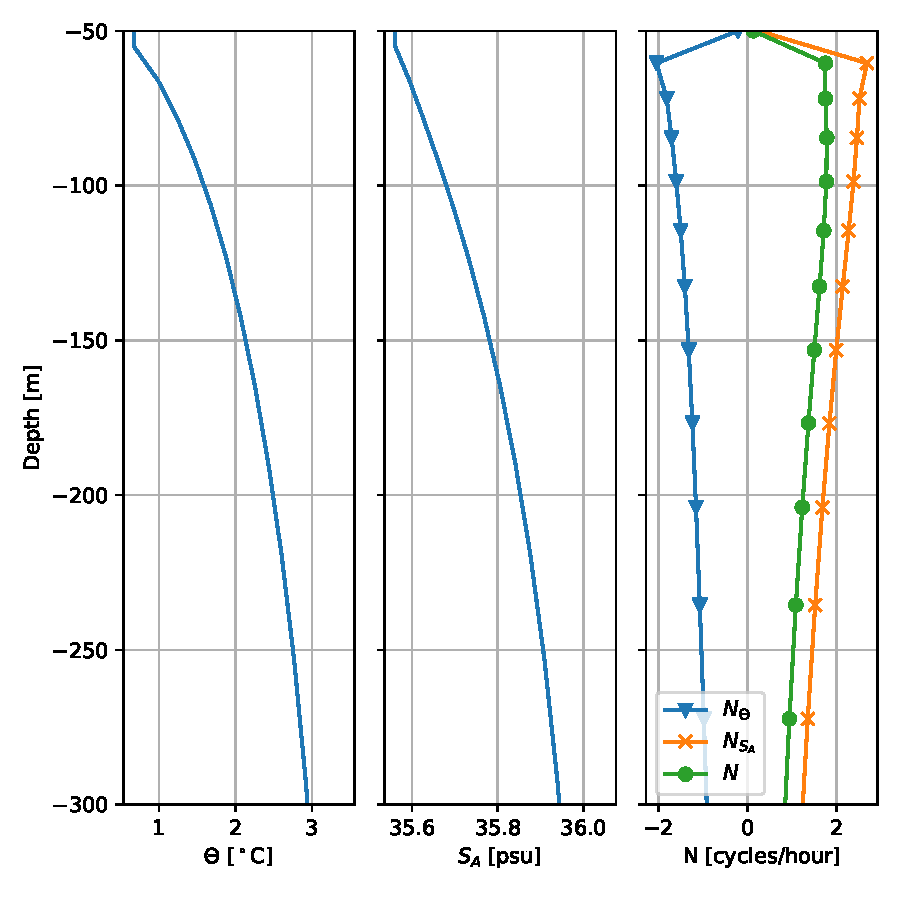
\includegraphics[width=7in]{strati}
      \caption{Temperature, salinity and buoyancy frequencies profiles
        in a beta-ocean ($19\,^\circ\text{E}$, $55\,^\circ\text{N}$).}
    \end{figure}


    \heading{Reference numerical values of the parameters}
    \vspace{-1.5cm}
    \begin{align*}
        C_b &= 9.851 \cdot 10^{-3} \text{\,kg}\text{\,m}^{-3}\text{\,K}^{-2} \\
        \Theta_0 &= -6.801\text{\,}^\circ\text{C} \\
        T_h &= 2.478 \cdot 10^{-5} \text{\,kg}\text{\,m}^{-4}\text{\,K}^{-1}\\
        %a_0 &= 1.655 \cdot 10^{-1} \text{\,kg\,m}^{-3}\text{\,K}^{-1} \\
        b_0 &= 7.6554 \cdot 10^{-1} \text{\,kg\,m}^{-3}\text{\,(g kg}^{-1}\text{)}^{-1} \\
        \rho_0 &= 1026 \text{\,kg\,m}^{-3} \\
        %T_0 &= 10\text{\,}^\circ\text{C}
    \end{align*}

    \heading{NEMO simplified EOS equivalence}% \emph{(ln\_seos=.true.)}}
    Implemented equation of state:
    \begin{align}
      \rho(\Theta, S_A, z) =
      \rho_0 -a_{0}\left(1+0.5 \lambda_1 \Delta\Theta+\mu_{1} z\right) \cdot \Delta\Theta
      +b_{0} \cdot \Delta S      
    \end{align}
    \begin{align*}
      \Delta\Theta = \Theta - 10 &\qand
      \Delta S = S_A - 35 \\
      C_b = a_0 \cdot \lambda_1 & \qand
      T_h = a_0 \cdot \mu_1 \\
      \Theta_0 = 10 - {1}/{\lambda_1} &\qand
      a_0 = 1.655 \cdot 10^{-1} \text{\,kg\,m}^{-3}\text{\,K}^{-1} 
    \end{align*}
    
  \end{exampleblock}

  %\vspace{2in}
  
  \begin{exampleblock}{xbasin and xnemogcm python packages}
    \heading{xnemogcm}
    \textbf{https://github.com/rcaneill/xnemogcm}
    \begin{itemize}
    \item Python package interfacing NEMO outputs to xgcm
    \end{itemize}
    
    \heading{xbasin}
    \textbf{https://github.com/rcaneill/xbasin}
    \begin{itemize}
    \item Python package used to deal with terrain-following coordinates
      on idealized configurations
    \item Based on NumPy, xarray, xgcm, f2py
    \end{itemize}

    \heading{Open source projects!}
    Please feel free to use, fork, and help on these new projects!
  \end{exampleblock}

  %\vspace{2in}
  
  \begin{block}{References}

    %\nocite{*}
    
    \footnotesize{
      \bibliographystyle{agufull08}
      \bibliography{poster}}

  \end{block}

\end{column}

\separatorcolumn
\end{columns}
\end{frame}

\end{document}
